\documentclass{article} %lots of other options here, like amsart, among others

% Preamble:

%Here's where packages go. 
\usepackage{amsmath} %includes lots of mathematical symbols and content
\usepackage{lipsum} % For blind text
\usepackage{fullpage}
%\usepackage[margin=1in]{geometry}
%\usepackage{geometry}
%\geometry{
%  top=1in,
%  inner=1in,
%  outer=1in,
%  bottom=1in,
%}
\usepackage{enumerate}
\usepackage{array,tabularx,multirow} %Helpful for certain tables and table features
\usepackage{graphicx}
\usepackage{wrapfig}
\graphicspath{ {./images/} }
\usepackage{float}
\usepackage{hyperref}%%Generally hyperref should be the last package loaded. 
%\hypersetup{
%    colorlinks=true,
%    urlcolor=blue,
%    linkcolor=black
%}

% To make typesetting augmented matrices easier. Code taken from
% https://tex.stackexchange.com/questions/2233/whats-the-best-way-make-an-augmented-coefficient-matrix 
\makeatletter
\renewcommand*\env@matrix[1][*\c@MaxMatrixCols c]{%
  \hskip -\arraycolsep
  \let\@ifnextchar\new@ifnextchar
  \array{#1}}
\makeatother

%%Custom Commands
\newcommand{\Z}{\mathbb{Z}}
\newcommand{\twobytwo}[4]{\begin{bmatrix} #1 & #2 \\ #3 & #4 \end{bmatrix}}

\title{Math 3680: Week 7}
\author{Arjan Singh Ellingson}
%\date{August 24th, 2026}
\date{\today}

\begin{document}

\maketitle
%\tableofcontents

\section{Picture of Moai}

This weekend I went for a 5 mile walk on Saturday. I have a lot of things I am thinking about and processing and I felt like just walking around aimlessly would help remedy from my stress. On my walk I was able to notice lots of things around SLO I had never noticed before. 
\vspace{0.5cm}
\begin{wrapfigure}{r}{0.35\textwidth}
    \centering
    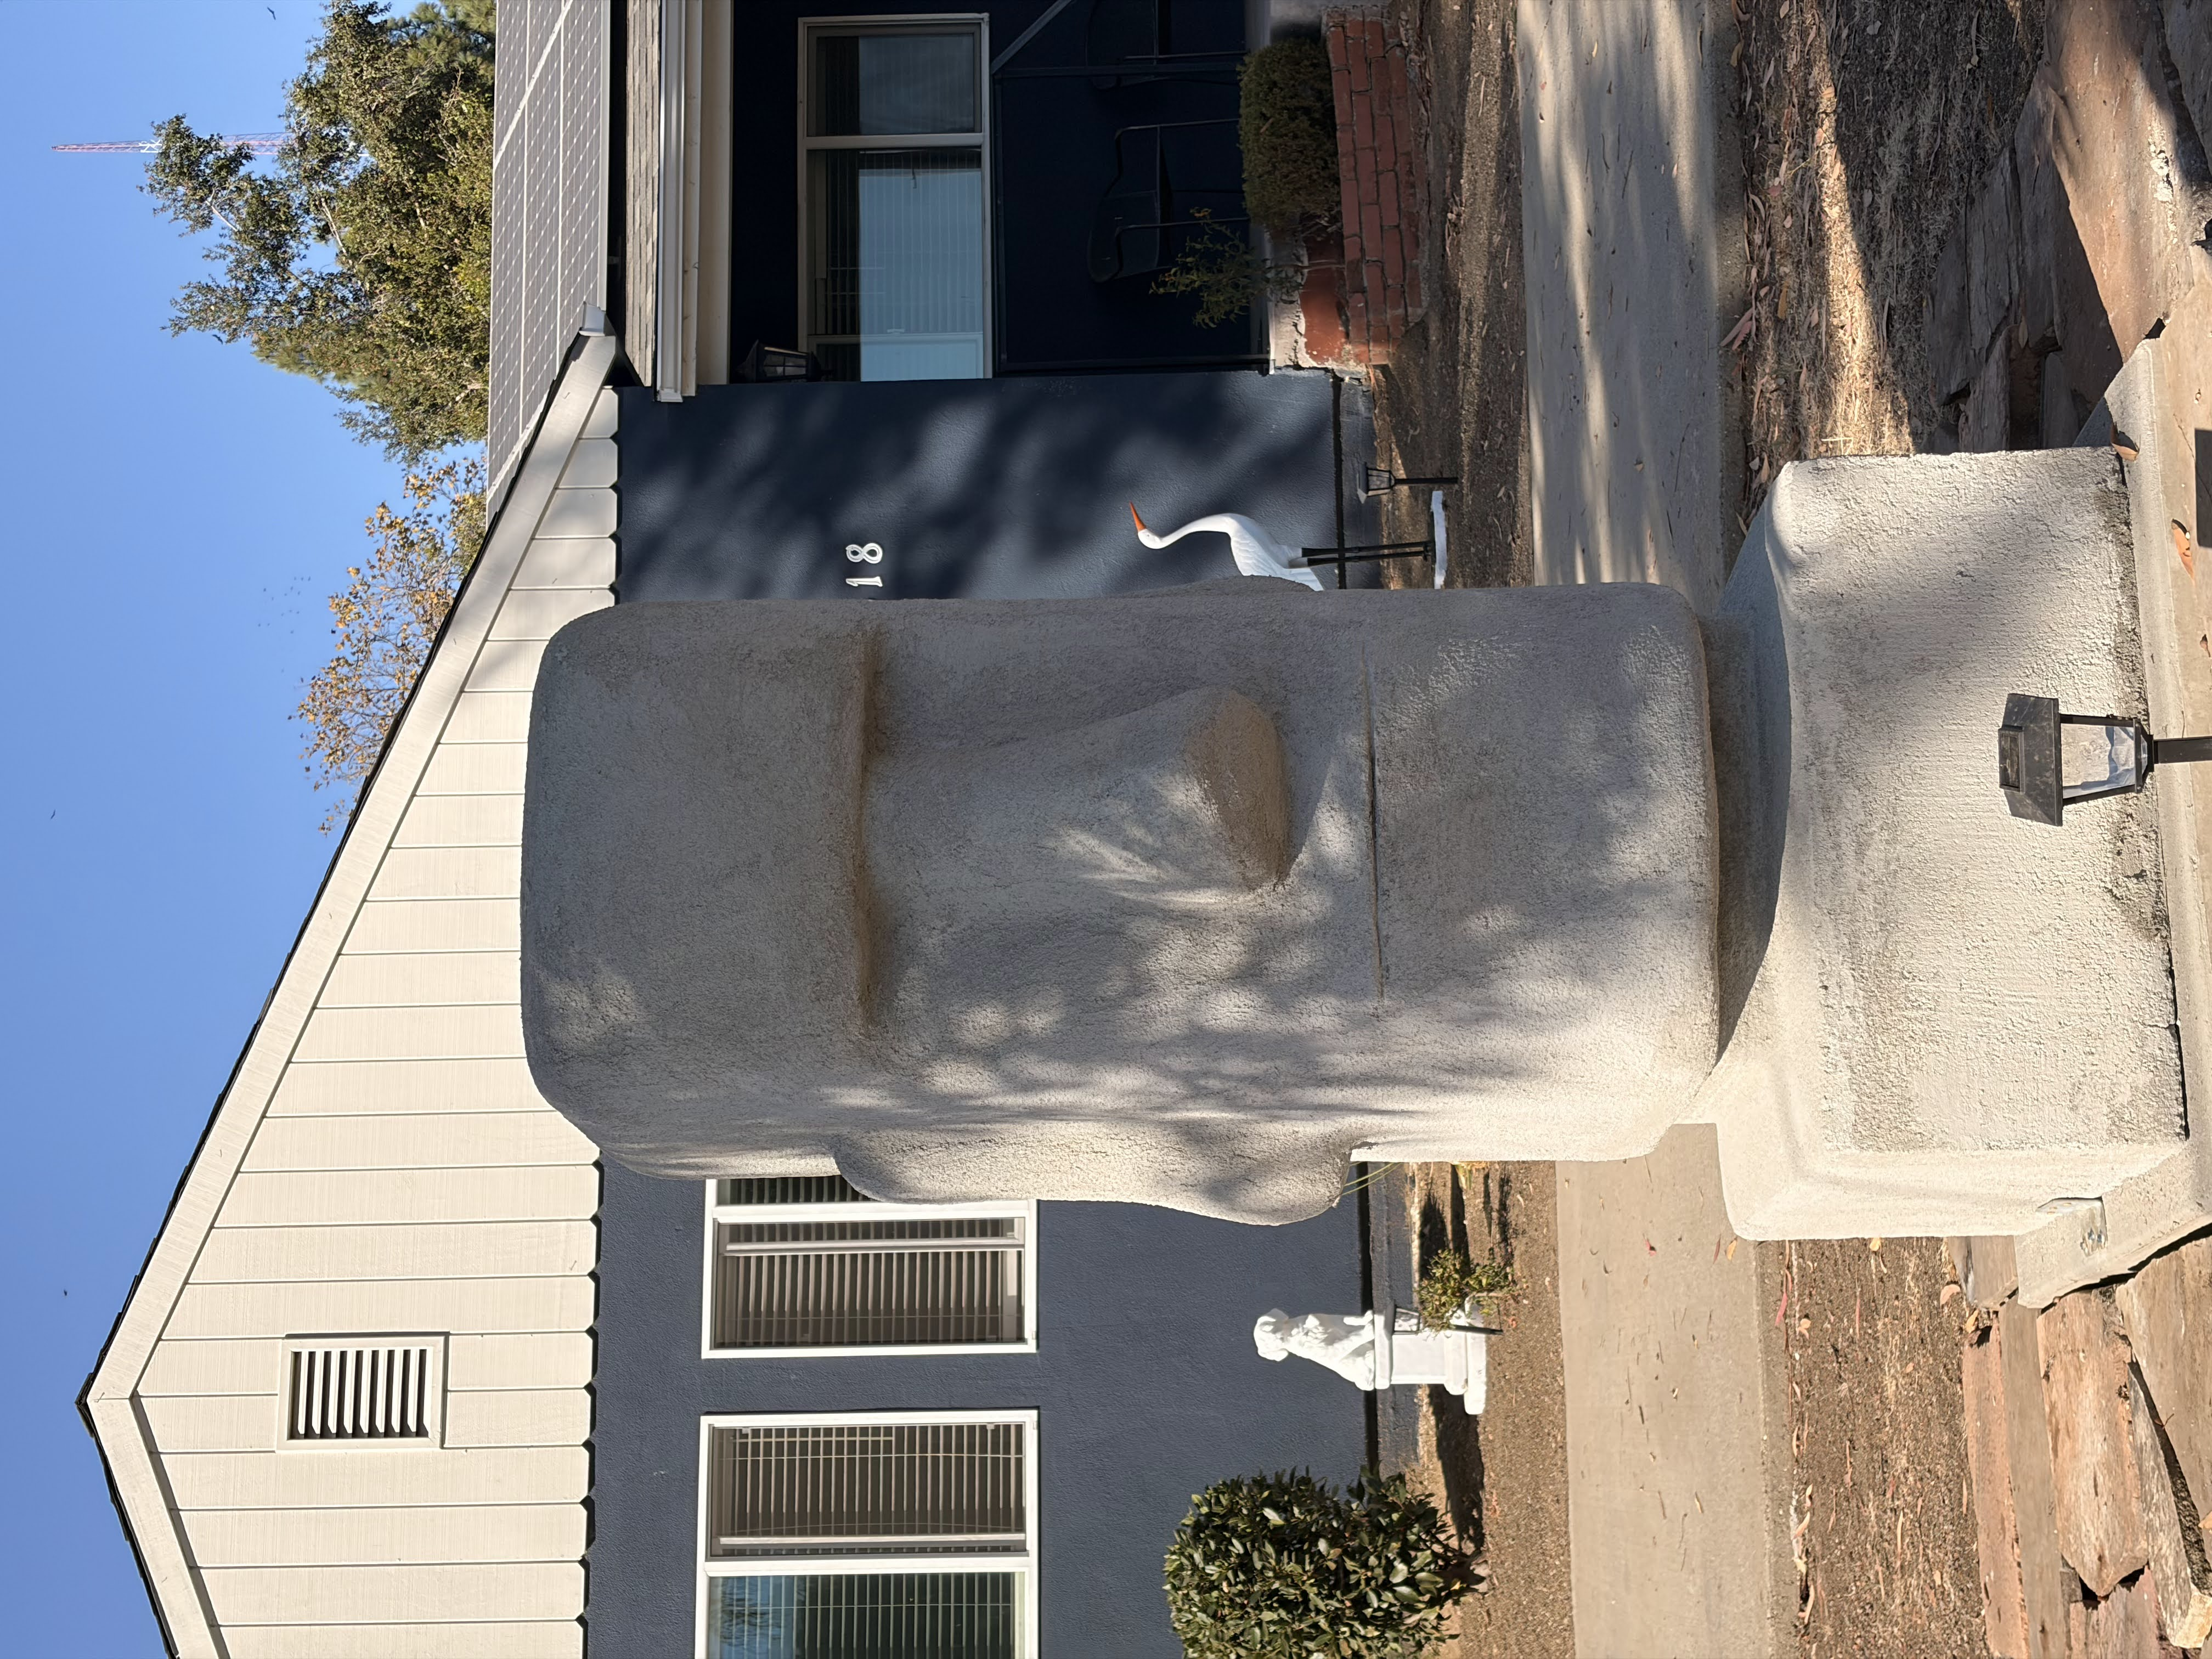
\includegraphics[width=0.9\linewidth, angle=-90]{Moai}
    \caption{A house with lots of statues and marble-like figures, found on highland.}
    \label{fig:moai_img}
\end{wrapfigure}
The first thing I ran into was a house with a lot of statues. It was somewhere along the highland neighborhood, but the garden was just filled with probably 10+ statues. The one that intrigued me the most was this Moai which was probably taller than me. 
\vspace{3cm}



Later on my walk I walked downtown along Broad Street, which is a walk I've done before that always has a lot of interesting houses and architecture along it. Lots of a flowers, too. This one in particular stood out to me, as it has vines. I am hoping to eventually in the future get vines tattooed along my arm so I waned to save this picture for reference.
\begin{figure}[H]
    \centering
    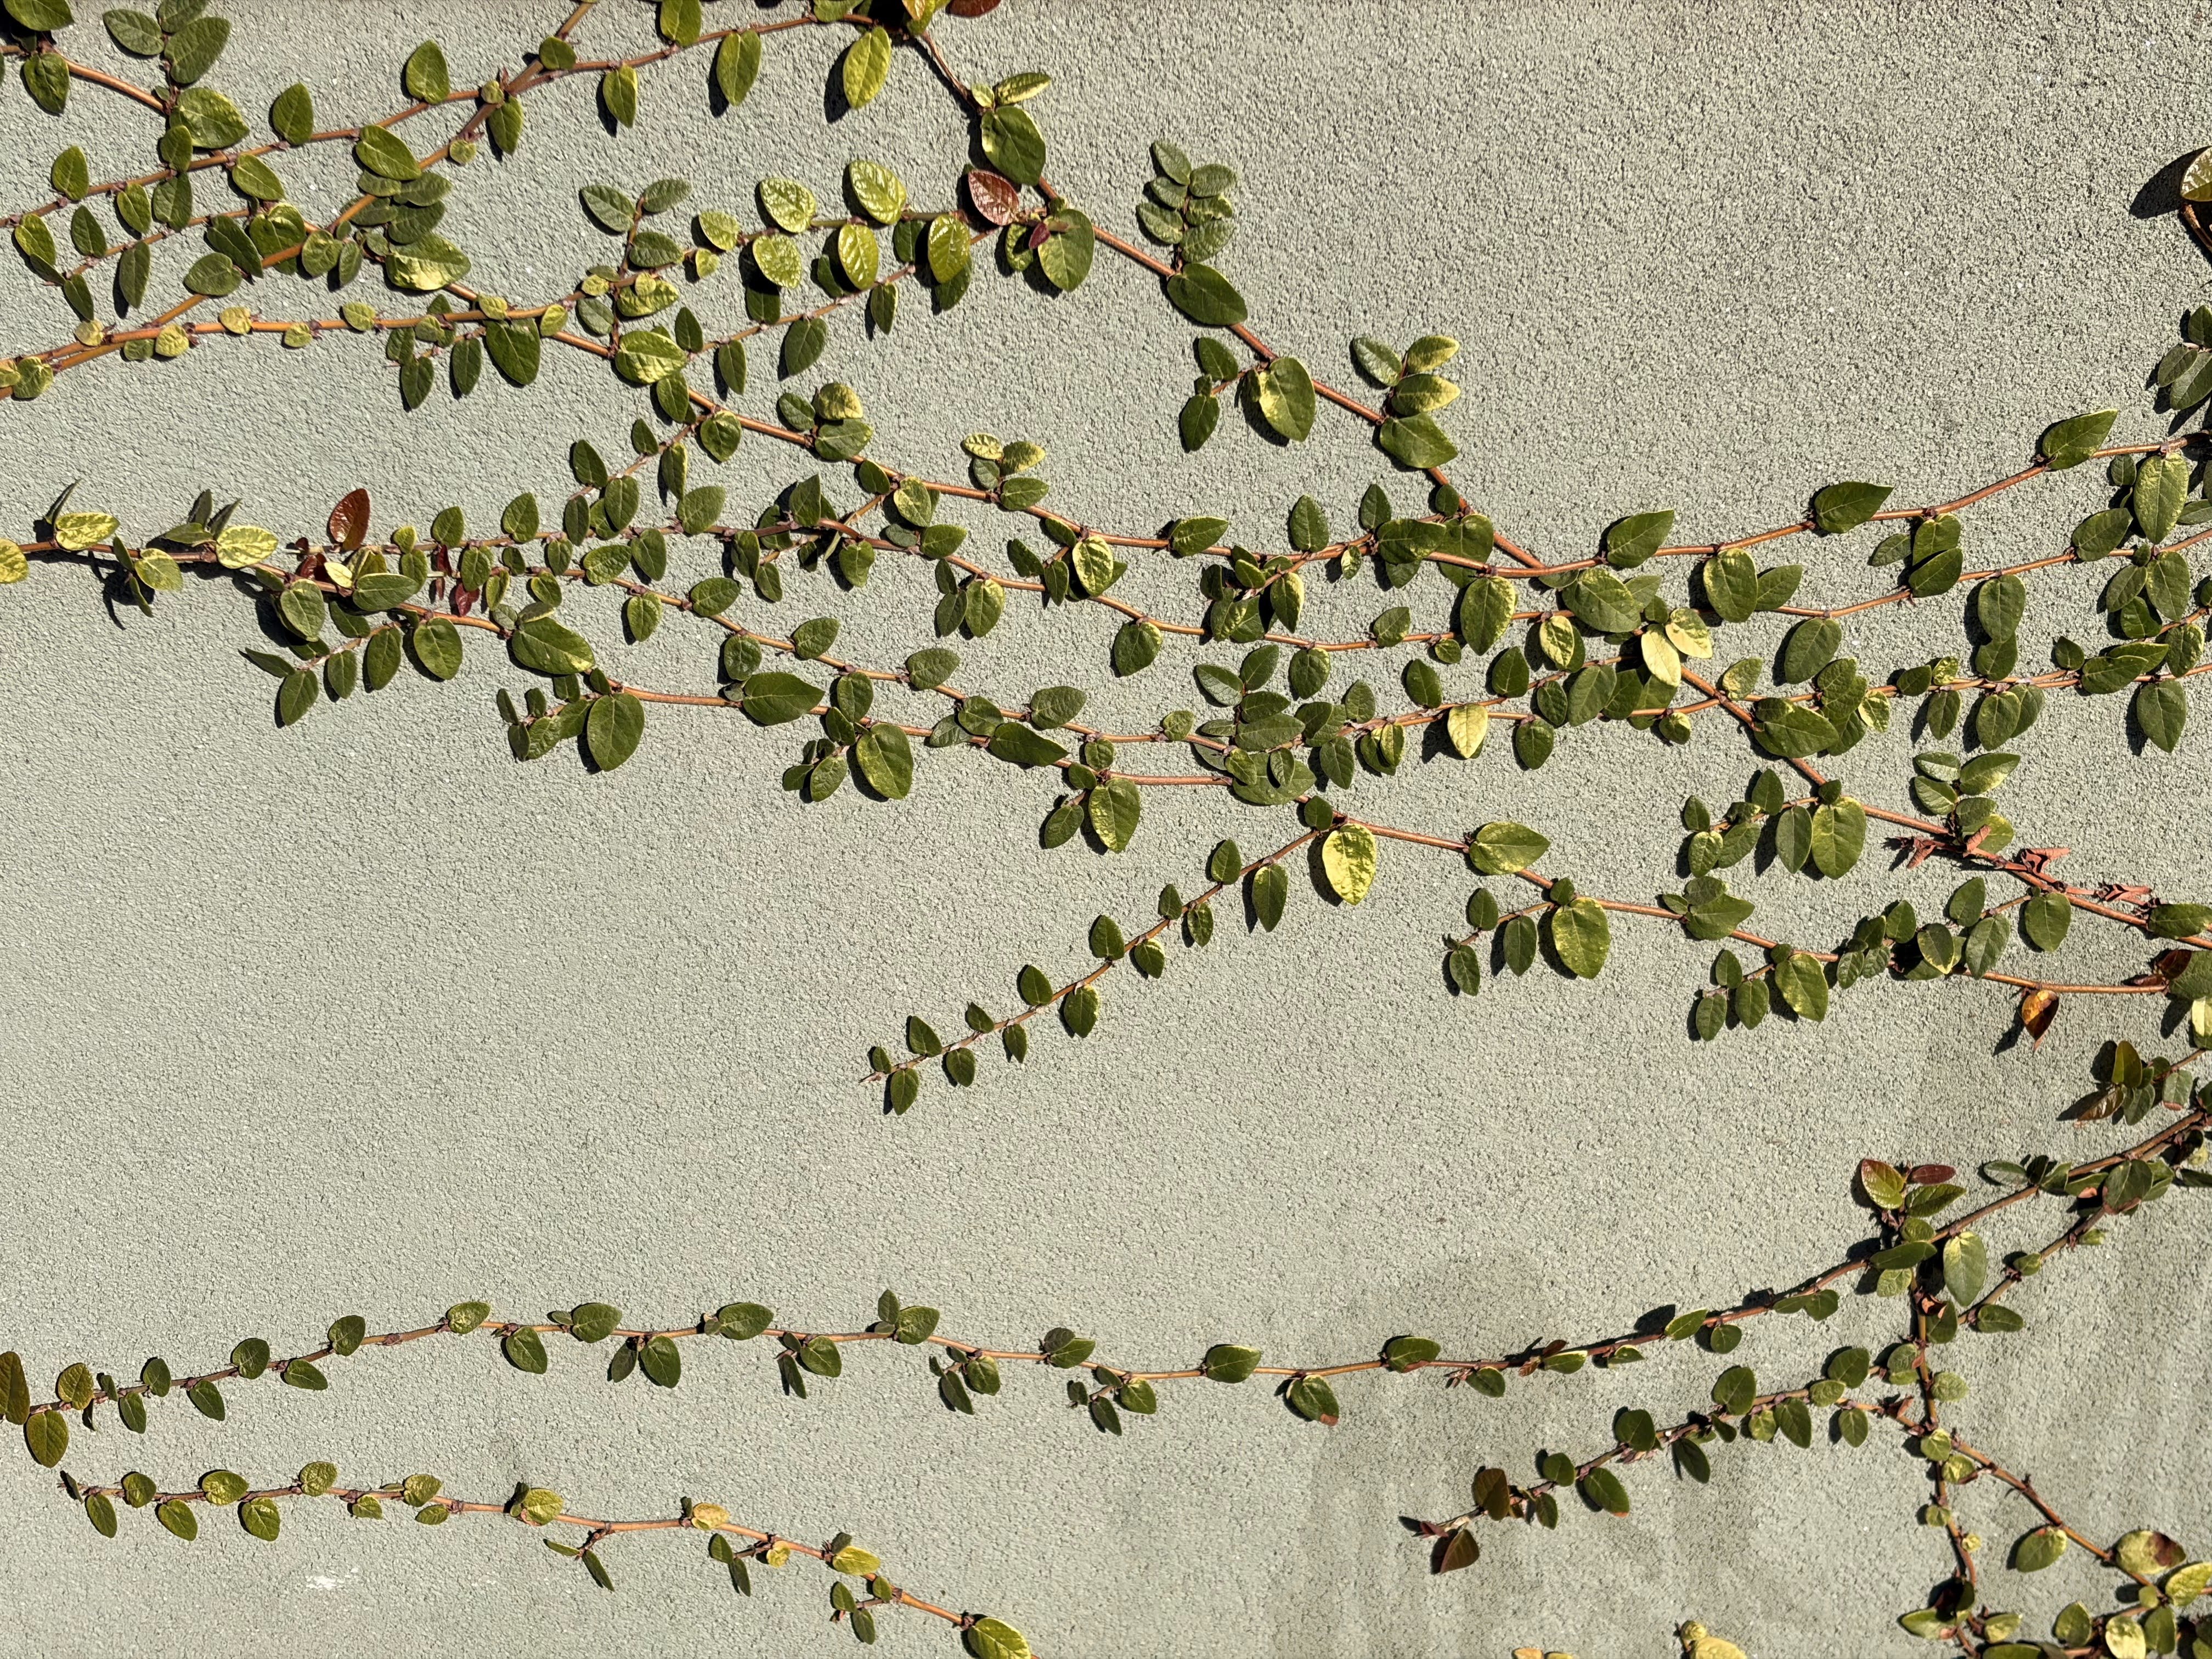
\includegraphics[width=0.65\textwidth]{Vines}
    \caption{Some vines along a house on Broad St.}
    \label{fig:vines_img}
\end{figure}


The last picture I want to include are some very pretty flowers along my walk. This was on the way back from Broad Street, growing kinda near a house on Foothill Hospital. 
\begin{figure}[H]
    \centering
    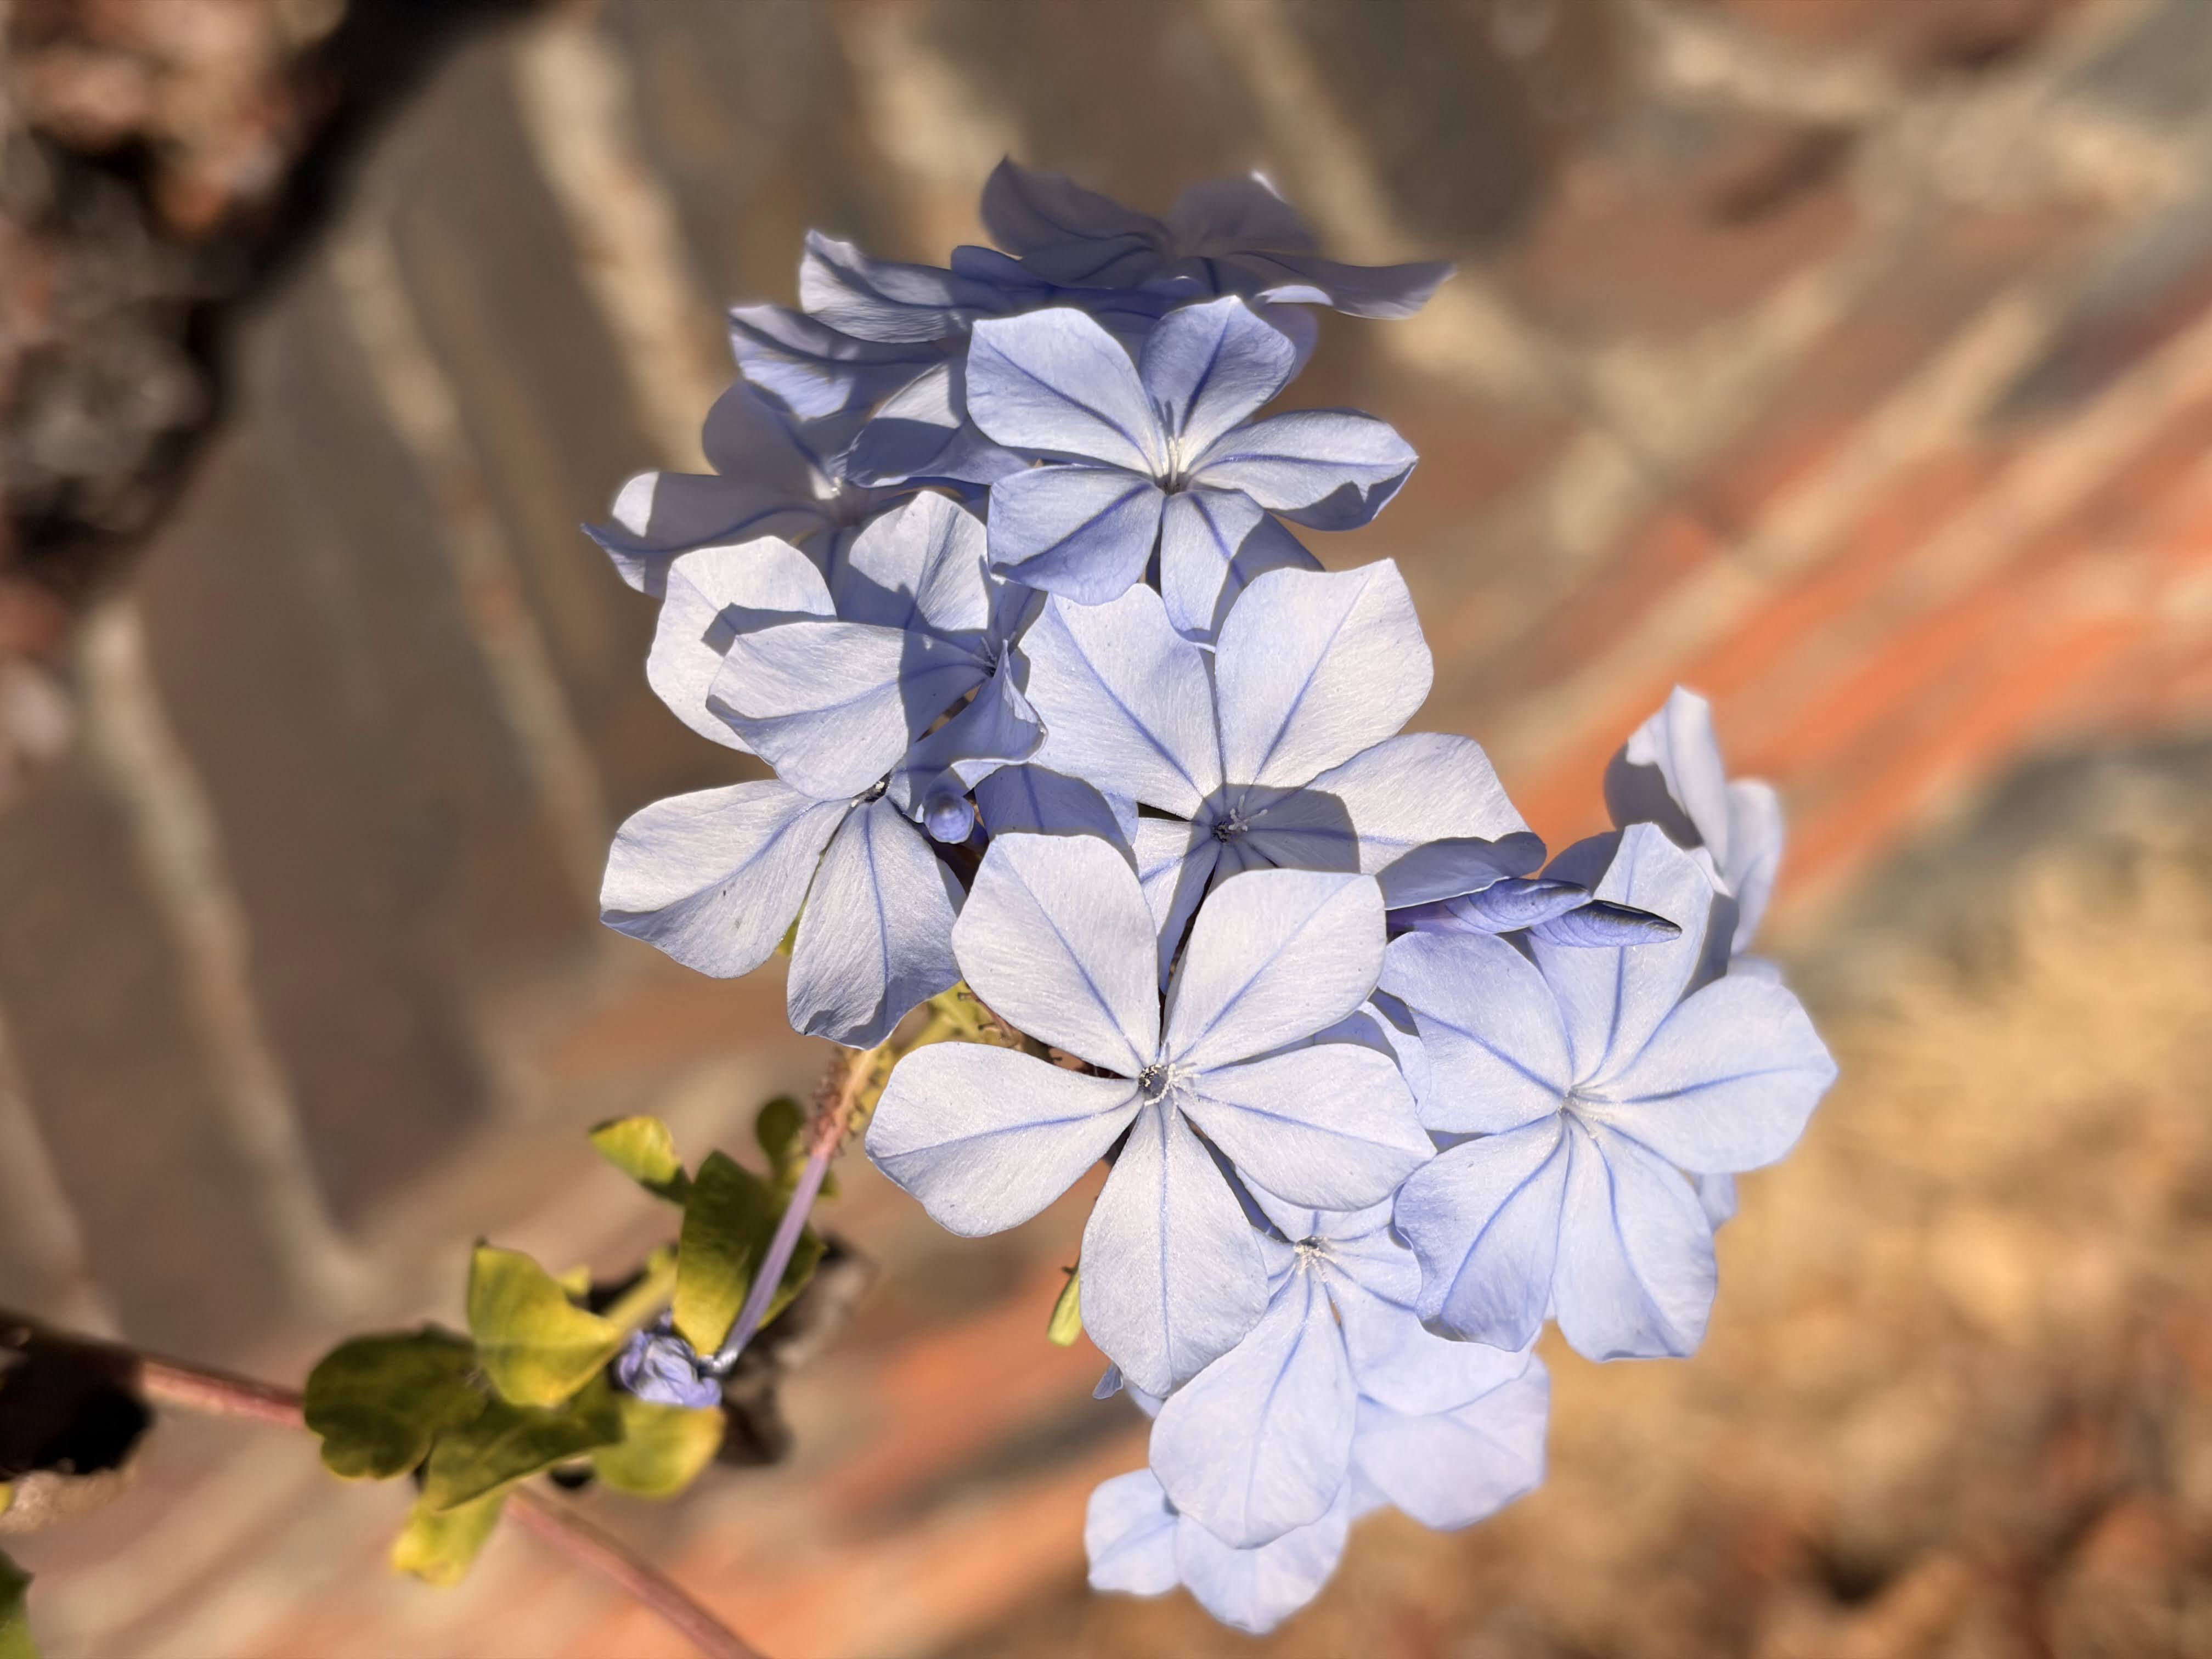
\includegraphics[width=0.8\textwidth]{Flowers}
    \caption{Very pretty blue (light purple?) flowers.}
    \label{fig:flowers}
\end{figure}
I did not know about the \texttt{\textbackslash listoffigures} command so this was cool to play with.
\listoffigures
\end{document}
